% Created 2016-08-17 Wed 14:38
\documentclass[tikz]{standalone}


\begin{document}
    \usetikzlibrary{arrows,positioning,decorations.pathmorphing}
    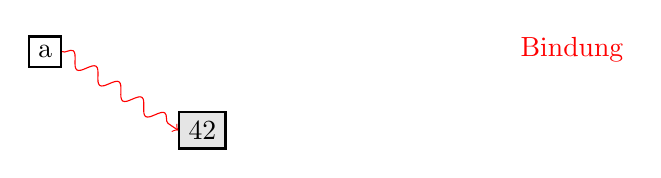
\begin{tikzpicture}
    [pyvariable/.style={rectangle,draw=black,thick},
     pyvalue/.style={rectangle,draw=black,fill=black!10,thick}]
    \node[pyvariable] (vara)  at (0,0) {a};
    \node[pyvalue] (val42) at (2,-1) {42};
    \draw [->,red,decorate,decoration=snake] (vara.east) -- (val42.west)
    node[right=5cm,above=0.75cm,]{Bindung};
    \end{tikzpicture}
\end{document}